\documentclass[../Main.tex]{subfiles}

\begin{document}
\author{Harmonics} %use author for title of lesson
\date{Year 1 Topic 19} %use date to refer to topic in main booklet

\section{Harmonics} %Section is the title of the lesson repeated, ready for the main contents page.

\begin{frame}{Waves on a string}
    If we attach a signal generator to a vibration generator to a length of string fixed at one end, we will produce a stationary wave -- this is a classic example of a stationary wave that exams love to include! 
    
    \begin{figure}
        \centering
        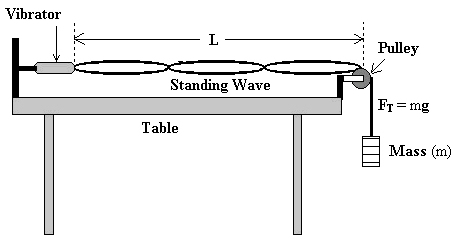
\includegraphics[height=4cm]{Waves_Images/vibrationgenerator.jpg}
    \end{figure}
    %Last lesson you gave it a go!
\end{frame}

\begin{frame}{Waves on a string}
A string will have a fundamental mode of vibration. Assuming both ends are fixed (or in other words have a node at each end), this will be produce a stationary wave appearing as a single "loop``. The frequency at which this happens is called the \emph{fundamental frequency}, denoted $f_0$.

\begin{figure}
    \centering
    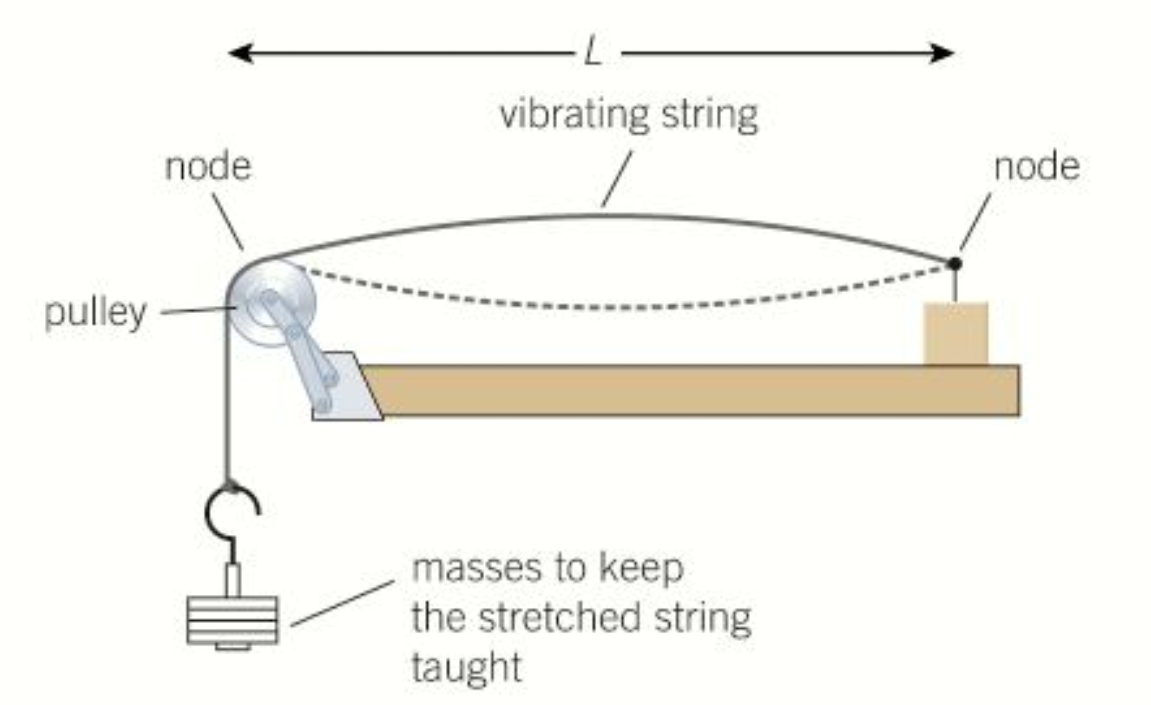
\includegraphics[height=3cm]{Waves_Images/1stharmonic.jpg}
\end{figure}
\pause
If the string has a length L, the wavelength of the wave produced at this fundamental frequency will be 2L. 
\end{frame}

\begin{frame}{First harmonic}
    Another name for this is the \emph{first harmonic}. This, of course, implies the existence of subsequent harmonics -- what do we think these might be? \pause
    
    \begin{block}{The harmonics}
    Are a series of specific frequencies that are integer multiples of the fundamental frequency. $f_n = n f_0$
    \end{block}
    
    Since the velocity of the wave is constant, if we change the frequency we change the wavelength, hence the harmonics appear as repeated "units``.
\end{frame}

\begin{frame}{The harmonics}
With an example of the first harmonic being 20Hz:
    \begin{figure}
        \centering
        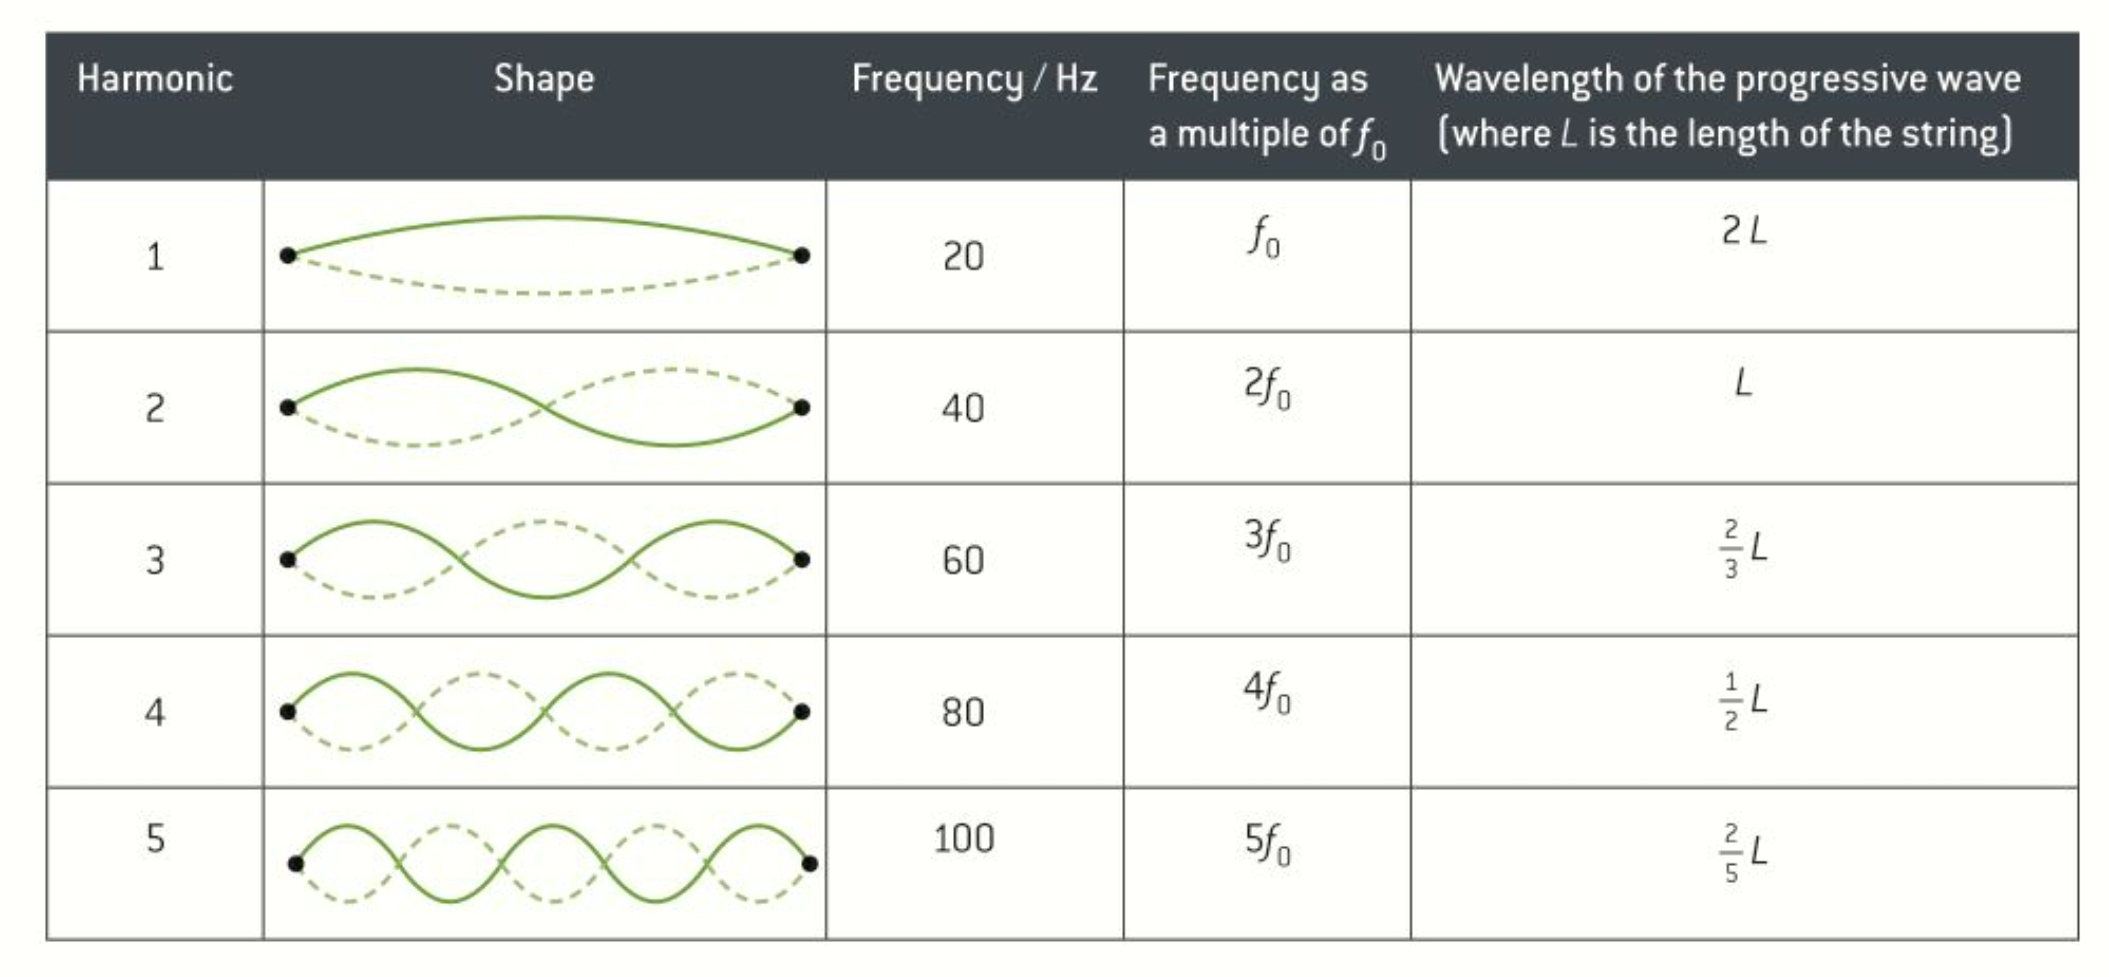
\includegraphics[width=\textwidth]{Waves_Images/theharmonics.jpg}
    \end{figure}
    Lets use this to try and work out the harmonics for this string! $[$Then Kerboodle page 232$]$
\end{frame}

\begin{frame}{String-based instruments}
    The principle of harmonics is exactly how guitars, pianos, violins etc. work. They have strings which will vibrate at a certain frequency. This frequency is tuned as one of the harmonics for that string, where the strings have a certain tension. 
    
    \begin{equation*}
        f_n = \frac{n}{2L}\sqrt{\frac{T}{\mu}}
    \end{equation*}
    
    Note that you do not need to know this formula, or ever use it for OCR, however it is good to know the variables that affect it: 
    \begin{itemize}
        \item L - the length of string
        \item T - tension in the string
        \item $\mu$ - the mass per unit length of string
    \end{itemize}
    \pause
    But how might a trumpet or another wind-based instrument work? They don't have strings...
\end{frame}

\begin{frame}{Wind-based instruments}
    In a closed tube with a single open end, a harmonic works slightly differently. At the closed end of the tube we see a node, at the open end we see an antinode.
    
    \begin{figure}
        \centering
        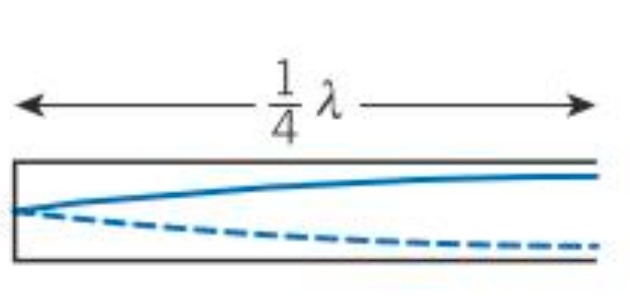
\includegraphics[width=4cm]{Waves_Images/open-closed_firstharmonic.jpg}
    \end{figure}
    The length of the tube gives $\frac{1}{4}\lambda$ -- or in other words, a full wavelength is 4L. 
    \pause
    \newline
    So what about the next harmonic, how might that look?
\end{frame}

\begin{frame}{Open-Closed Tube}
    The other harmonics for sound are as follows, where we instead only look at odd-integer values of harmonics:
    \begin{multicols}{2}
    \begin{figure}
        \centering
        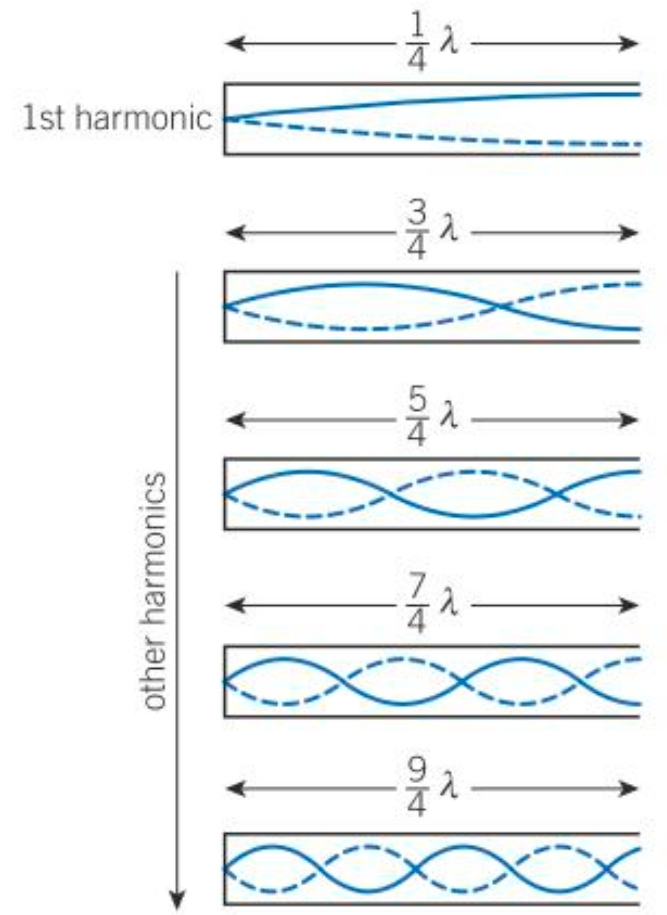
\includegraphics[height=6cm]{Waves_Images/open-closed_harmonics.jpg}
    \end{figure}
    \columnbreak
    You could be expected to be able to deduce the wavelength given a length of tube.
    
    \begin{minipage}{5.5cm}
    \begin{exampleblock}{Example}
    A sound plays in a flute on the third harmonic. If the length of the flute is 33cm, determine the wavelength, and hence frequency of the sound produced.
    \end{exampleblock}
    (speed of sound in air = 340m/s)
    \end{minipage}
    \end{multicols}
\end{frame}

\begin{frame}{Open-Open Tubes}
    \begin{multicols}{2}
    With a tube open at both ends we can have every integer harmonic, with antinodes at both ends of the tube. 
    \newline
    
    A common question is to be given a tube and to label nodes and antinodes, or determine the wavelength from these.
    \columnbreak
    \begin{figure}
        \centering
        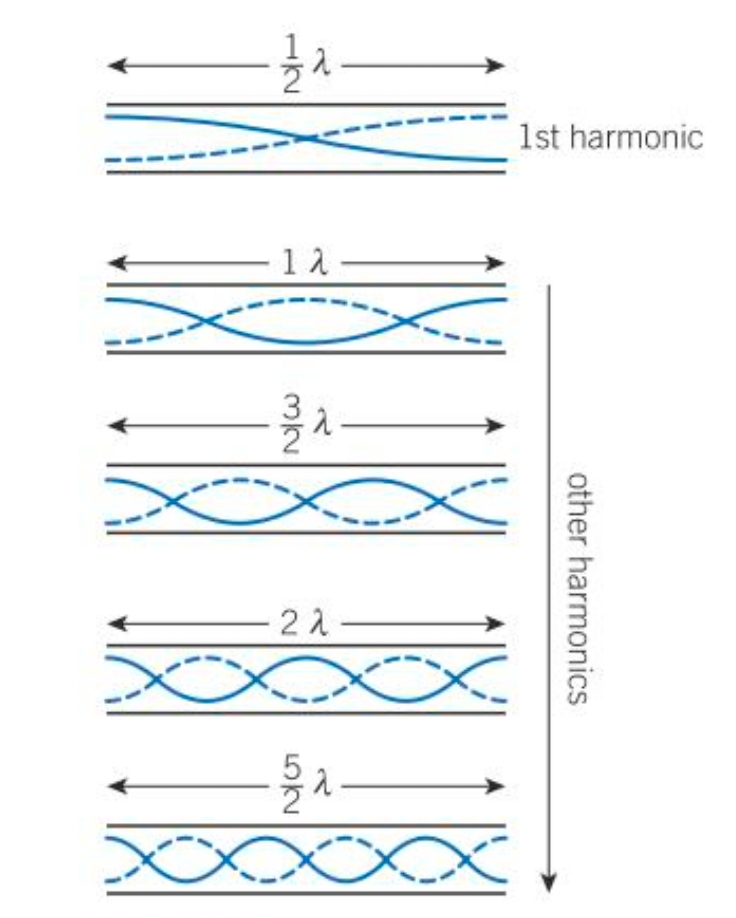
\includegraphics[height=6cm]{Waves_Images/open-open_harmonics.jpg}
    \end{figure}
    \end{multicols}
    \pause 
    $[$and now: Kerboodle page 235$]$
\end{frame}

\end{document}